\documentclass[xcolor=dvipsnames,10pt,aspectratio=169]{beamer}
%\usetheme[hideallsubsections]{Hannover}
\usetheme[width=1.75cm]{Hannover} % plenty of themes to pick from
\graphicspath{{../../images/}}
\usepackage[utf8]{inputenc}
\usepackage[T1]{fontenc}
\usepackage{amsmath}
\usepackage{amsfonts}
\usepackage{amssymb}
\usepackage{graphicx,hyperref,url}
\usepackage{textpos}
\usepackage{multicol}
\usepackage{bm}
\usepackage{tikz}
\usepackage{verbatim}
\usepackage{braket}
\usetikzlibrary{arrows,shapes}
\usecolortheme{crane} % plenty of color themes to pick from
\useinnertheme{rectangles}

\definecolor{UBCgreen}{RGB}{30, 77, 43} % UBC Blue (primary)
\definecolor{UBCgold}{RGB}{200, 195, 114} % UBC Grey (secondary)

\setbeamercolor{palette primary}{bg=UBCgreen,fg=white}
\setbeamercolor{palette secondary}{bg=UBCgreen,fg=white}
\setbeamercolor{palette tertiary}{bg=UBCgreen,fg=white}
\setbeamercolor{palette quaternary}{bg=UBCgreen,fg=white}
\setbeamercolor{palette sidebar primary}{fg=UBCgreen,bg=UBCgold}
\setbeamercolor{palette sidebar secondary}{fg=UBCgreen,bg=UBCgold}
\setbeamercolor{palette sidebar tertiary}{fg=UBCgreen,bg=UBCgold}
\setbeamercolor{palette sidebar quaternary}{fg=UBCgreen,bg=UBCgold}
\setbeamercolor{structure}{fg=UBCgreen} % itemize, enumerate, etc
\setbeamercolor{section in toc}{fg=UBCgreen} % TOC sections
\setbeamercolor{subsection in head/foot}{bg=UBCgold,fg=white}
\setbeamercolor{section in sidebar}{fg=UBCgreen}
\setbeamercolor{section in sidebar}{fg=UBCgreen}
\setbeamertemplate{page number in head/foot}[totalframenumber]
\setbeamertemplate{navigation symbols}{\footnotesize\usebeamertemplate{page number in head/foot}}
\setbeamertemplate{frametitle}[default][left,colsep=-4bp,rounded=false]
\setbeamertemplate{section in toc}[bullets]
%\addtobeamertemplate{frametitle}{}{%
%    \begin{textblock*}{100mm}(0.95\textwidth,-0.95cm)
%    
\includegraphics[width=0.925cm]{CSU-Ram-357-617.pdf}
%    \end{textblock*}
%}
\makeatletter
\setbeamertemplate{sidebar canvas \beamer@sidebarside}%
                  [vertical shading][top=UBCgold,bottom=UBCgold]
\makeatother

\addtobeamertemplate{sidebar left}{}{
  \hspace{0.3cm}
  \vspace{0.2cm}
  
\includegraphics[align = l, width = 1cm]{CSU-Ram-357-617.pdf}
}

%\setbeamertemplate{section in toc}{\hspace*{0em}\inserttocsection}
%\setbeamertemplate{subsection in toc}{\hspace*{2em}\inserttocsubsection}

\newcommand{\ham}{\mathcal{H}}
\newcommand{\TT}{Transition from 2D to a 1D topological superconductivity in a triangular p-wave superconductor island}
\newcommand{\ST}{Transtition from 2D to a 1D topological p-wave superconductor }
\newcommand{\MO}{Motivation}
\newcommand{\PW}{P-wave superconductors and Braiding}
\newcommand{\EF}{Effective p-wave and triangular islands}
\newcommand{\FO}{Formulation}
\newcommand{\RE}{Results}
\newcommand{\CO}{Summary}

\title[\ST]{\TT}
\subtitle{}
\author[Aidan Winblad]{Aidan Winblad \small \and\\ Hua Chen}
\institute{Department of Physics \and\\ Colorado State University}
\date{\small\today}

\begin{document}

  \begin{frame}
  \titlepage
  \end{frame}

  \begin{frame}
  \frametitle{Outline}
    \begin{itemize}
      \item \MO
        \begin{itemize}
          \item \PW
          \item \PE
        \end{itemize}
      \item \FO
      \item \RE
        \begin{itemize}
          \item 
          \item 
        \end{itemize}
      \item \CO
    \end{itemize}
  \end{frame}

  \section{\MO}
  \begin{frame}{\MO}{}

    \begin{multicols}{2}

    \begin{itemize}
      \item P-wave superconductors exhibit non-Abelian statistices by braiding half-quantum vortices.
        \begin{itemize}
          \item Majorana fermions located at core of a vortex.
        \end{itemize}
      \item 1D p-wave superconductors host Majorana fermions at end points.
        \begin{itemize}
          \item Measured in real systems using effective p-wave superconductors.
          \item Mourik, \textit{Science} \textbf{336}, 1003 (2012).
          \item Nadj-Perge, \textit{Science} \textbf{346}, 602 (2014).
        \end{itemize}
      \item Quasi-1D T-junction.
        \begin{itemize}
          \item Non-Abelian statistics of Majorana fermions is meaningful only in 2D.
          \item In practice challenging to make T-junction networks.
        \end{itemize}
    \end{itemize}

    \begin{figure}
      \begin{tikzpicture}
        \node[inner sep=0pt] (figure) at (0,0)
        {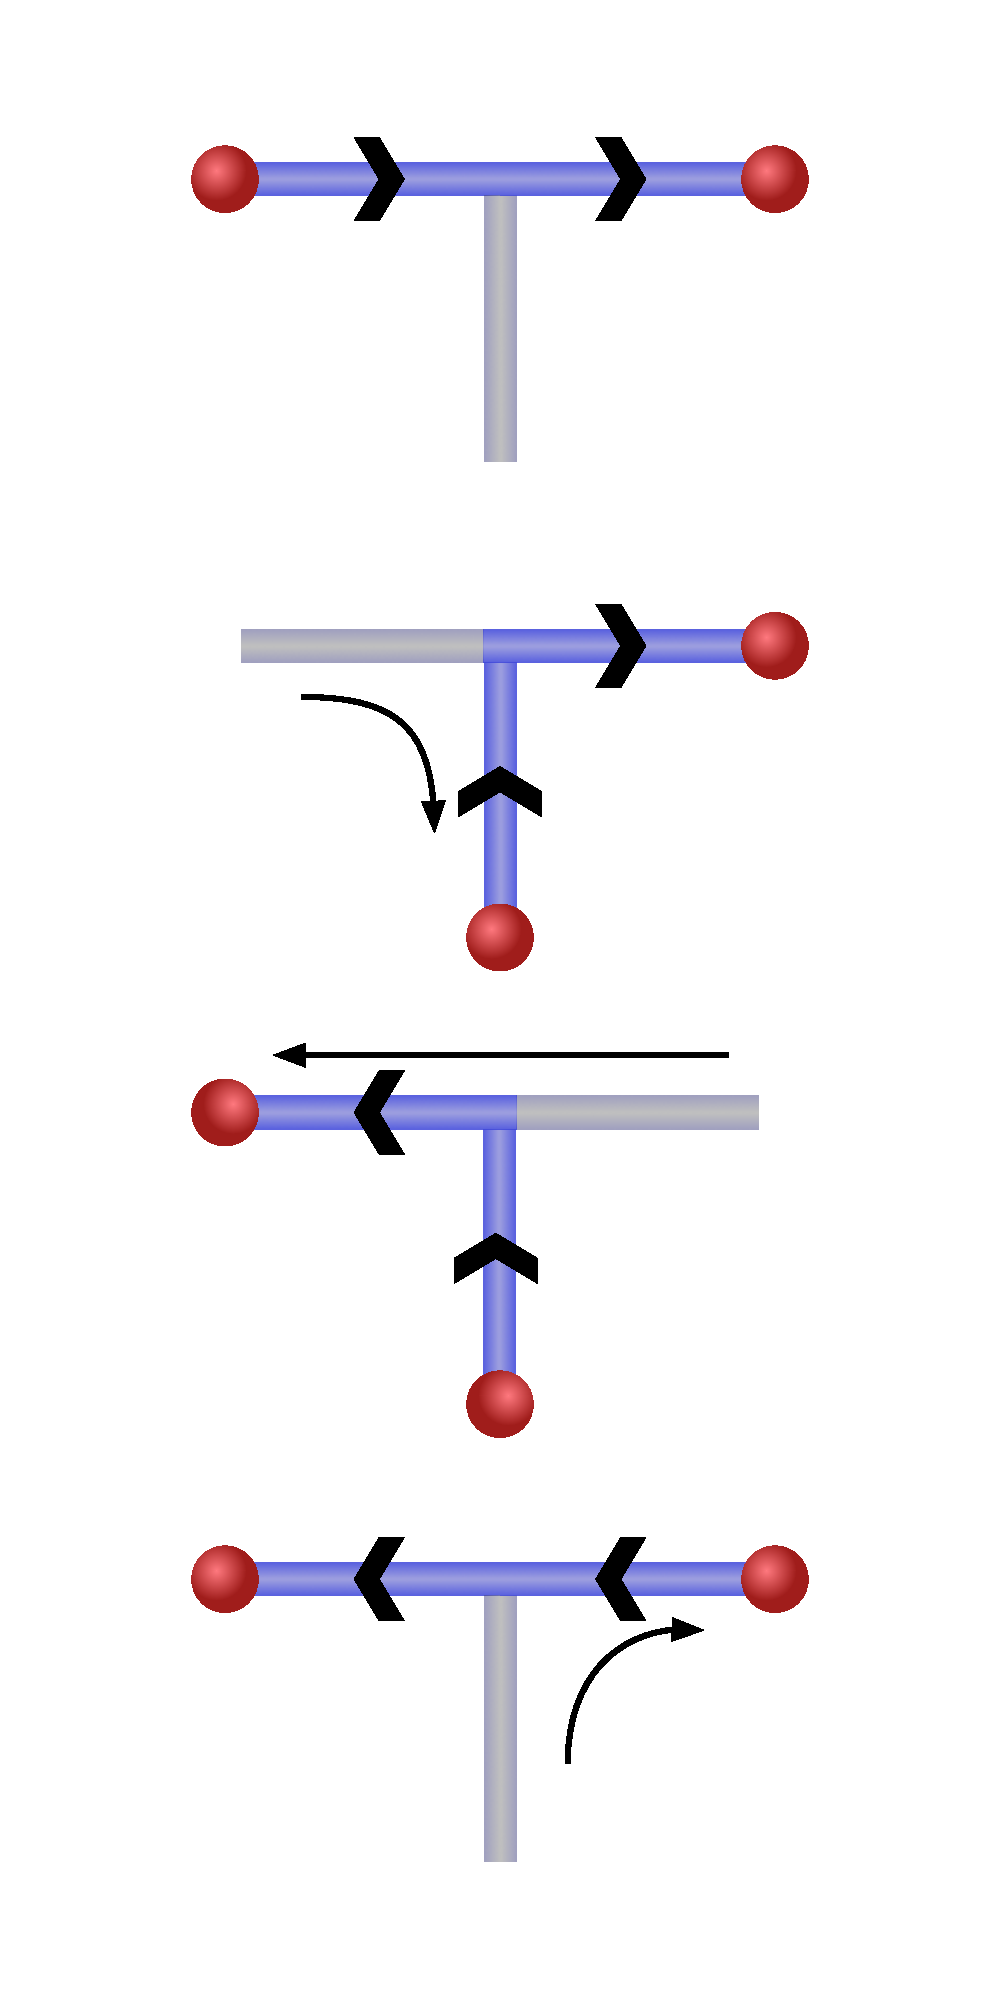
\includegraphics[width=0.25\textwidth]{../../images/t-junction.pdf}};
        \node[inner sep=0pt] (caption) at (0,-3.2) {\small Alicea, \textit{Nature Phys.} \textbf{7}, 412 (2011)}
        \end{tikzpicture}
      \end{figure}
    \end{multicols}

  \end{frame}

  \begin{frame}
    \frametitle{\MO}
    \begin{multicols}{2}

    \begin{itemize}
      \item Consider triangular islands, topologically similar to T-junctions.
      \item Islands of three-fold rotational symmetry occur naturally in epitaxial growth on close-packed metal surfaces.
      \item Triangular Co islands on Cu(111).
      \item Good platform for transition from 2D to a 1D topological superconductor.
    \end{itemize}
    \newline

    \begin{figure}
      \begin{tikzpicture}
        \node[inner sep=0pt] (figure) at (0,0)
        {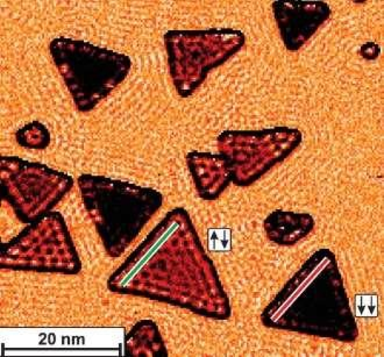
\includegraphics[width=0.4\textwidth]{../../images/triangular-islands.pdf}};
        \node[inner sep=0pt] (caption) at (0,-3.2) {\small Pietzsch, \textit{PRL} \textbf{96}, 237202 (2006)}
        \end{tikzpicture}
      \end{figure}
    \end{multicols}

  \end{frame}

  \section{\FO}
  \begin{frame}
    \frametitle{Tunable superconductor device}

    \begin{multicols}{2}
      \begin{figure}
        \begin{tikzpicture}
          \node[inner sep=0pt] (figure) at (0,0)
          {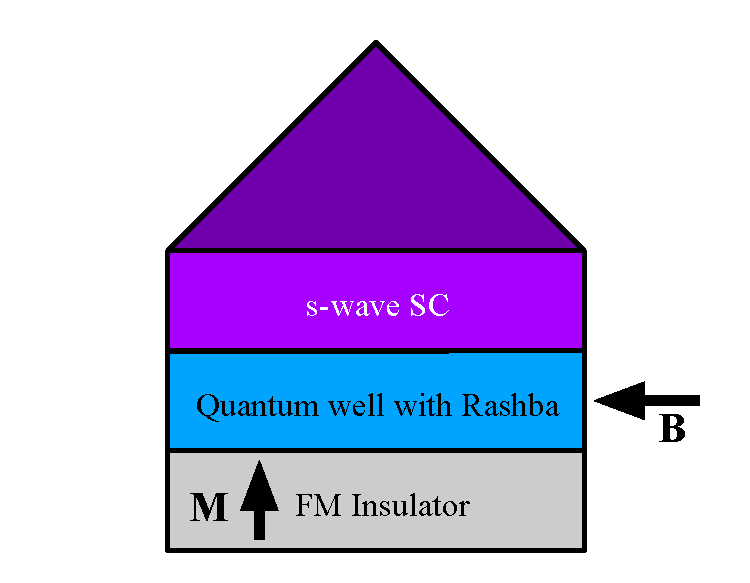
\includegraphics[width=0.5\textwidth]{../../images/tunable-semiconductor.pdf}};
          \node[inner sep=0pt] (caption) at (0,-3.2) {\small Alicea, \textit{PRB} \textbf{81}, 125318 (2010)}
          \end{tikzpicture}
        \end{figure}

    Effective p-wave Hamiltonian:
    \begin{align}
      &\ham_{eff} = \ham_0 + \ham_Z + \ham_{SC} + \ham_R \notag\\
      &\ham_0 = \sum_j (6t - \mu) c_j^{\dagger} c_j -\sum_{\braket{j,k}} (t c_j^{\dagger} c_k + h.c.) \notag\\
      &\ham_Z = \sum_j c_j^{\dagger} \bm{V} \cdot \bm{\sigma} c_j \notag  \\
      &\ham_{SC} = \sum_j (\Delta c_{j\uparrow}^{\dagger} c_{j\downarrow}^{\dagger} + h.c) \notag \\
      &\ham_R = -it_R\sum_{\braket{j,k}}  c_j^{\dagger} \bm{\sigma} \times \bm{r}_{jk} \cdot \hat{\bm{z}}_k c_j \notag
    \end{align}
    \end{multicols}

  \end{frame}

  \section{\RE}
  \begin{frame}
    \frametitle{Zero in-plane Zeeman field}

    \begin{figure}
      \begin{tikzpicture}
        %\draw[help lines,gray!20] (-4,-4) grid[step=0.5] (4,4);
        \node[inner sep=0pt] (figure) at (-3,0)
        {\includegraphics[width=0.5\textwidth]{../../images/wavefunction-1.pdf}};
        \node[inner sep=0pt] (figure) at (2.5,0)
        {\includegraphics[width=0.5\textwidth]{../../images/wavefunction-2.pdf}};
        %\node[inner sep=0pt] (figure) at (3,0) {a figure}
      \end{tikzpicture}
    \end{figure}

  \end{frame}

  \begin{frame}
    \frametitle{Nonzero in-plane Zeeman field}

    \begin{figure}
      \begin{tikzpicture}
        %\draw[help lines,gray!20] (-4,-4) grid[step=0.5] (4,4);
        \node[inner sep=0pt] (figure) at (-3,0)
        {\includegraphics[width=0.5\textwidth]{../../images/wavefunction-1-in-plane.pdf}};
        \node[inner sep=0pt] (figure) at (2.5,0)
        {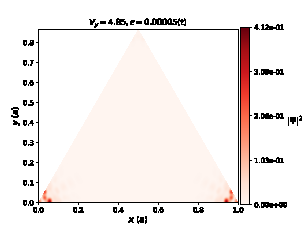
\includegraphics[width=0.5\textwidth]{../../images/wavefunction-2-in-plane.pdf}};
        %\node[inner sep=0pt] (figure) at (3,0) {a figure}
      \end{tikzpicture}
    \end{figure}
  \end{frame}

  \begin{frame}
    \frametitle{DOS spectral flow}

    \begin{figure}
      \begin{tikzpicture}
        %\draw[help lines,gray!20] (-4,-4) grid[step=0.5] (4,4);
        \node[inner sep=0pt] (figure) at (0,0)
        {\includegraphics[width=.75\textwidth]{../../images/spectral-flow-dos.pdf}};
      \end{tikzpicture}
    \end{figure}
  \end{frame}

  \begin{frame}
    \frametitle{DOS at the vertices}

    \begin{figure}
      \begin{tikzpicture}
        %\draw[help lines,gray!20] (-4,-4) grid[step=0.5] (4,4);
        \node[inner sep=0pt] (figure) at (-3,0)
        {\includegraphics[width=0.5\textwidth]{../../images/dos-upper-vertex.pdf}};
        \node[inner sep=0pt] (figure) at (2.5,0)
        {\includegraphics[width=0.5\textwidth]{../../images/dos-lower-vertex.pdf}};
        %\node[inner sep=0pt] (figure) at (3,0) {a figure}
      \end{tikzpicture}
    \end{figure}
  \end{frame}

  \begin{frame}
    \frametitle{A closer look}

    \begin{figure}
      \begin{tikzpicture}
        %\draw[help lines,gray!20] (-4,-4) grid[step=0.5] (4,4);
        \node[inner sep=0pt] (figure) at (-3,0)
        {\includegraphics[width=0.5\textwidth]{../../images/dos-upper-vertex-zoomed.pdf}};
        \node[inner sep=0pt] (figure) at (2.5,0)
        {\includegraphics[width=0.5\textwidth]{../../images/dos-lower-vertex-zoomed.pdf}};
        %\node[inner sep=0pt] (figure) at (3,0) {a figure}
      \end{tikzpicture}
    \end{figure}
  \end{frame}

  \section{\CO}
  \begin{frame}
    \frametitle{Summary}
    \begin{itemize}
      \item Numerical effects due to finite size do not give exact zero energy wavefunctions.
      \item Introduction of in-plane Zeeman field breaks the three-fold symmetry yielding two-fold symmetry.
      \item Next steps
        \begin{itemize}
          \item Complete analytical description of corner states.
          \item Infinite wedge.
          \item Develop robust braiding formulation.
        \end{itemize}
    \end{itemize}
  \end{frame}


%  \begin{frame}
%  \frametitle{List}
%  \begin{itemize}
%  \item Point A
%  \item Point B
%  \begin{itemize}
%  \item part 1
%  \item part 2
%  \end{itemize}
%  \item Point C
%  \item Point D
%  \end{itemize}
%  \end{frame}
%
%  \begin{frame}
%    \frametitle{Enumerate}
%    \begin{enumerate}[]
%  \item Point A
%  \item Point B
%  \begin{enumerate}[i]
%  \item part 1
%  \item part 2
%  \end{enumerate}
%  \item Point C
%  \item Point D
%  \end{enumerate}
%  \end{frame}
%
%  \begin{frame}
%  \frametitle{Using Columns}
%    \begin{columns}
%      \column{0.5\textwidth}
%      Lorem ipsum dolor sit amet, consectetur adipisicing elit, sed do eiusmod tempor incididunt ut labore et dolore magna aliqua.
%      \column{0.5\textwidth}
%      Lorem ipsum dolor sit amet, consectetur adipisicing elit, sed do eiusmod tempor incididunt ut labore et dolore magna aliqua.
%    \end{columns}
%  \end{frame}

\end{document}


